\documentclass[a4paper]{article}

\usepackage[english]{babel}
\usepackage[utf8]{inputenc}
\usepackage{amsmath}
\usepackage{graphicx}
\usepackage{enumerate}
\usepackage{eqnarray}

\textheight=10in
\textwidth=6.9in
\topmargin=0.0in
\headheight=-0.3in
\headsep=-0.3in
\leftmargin=-0.2in
\rightmargin=-0.4in
\oddsidemargin=-0.3in
\evensidemargin=-0.5in
\parindent=0.0in

\pagestyle{empty}

\def\dd{\Delta}
\def\ss{\displaystyle\sum}
\def\lb{\left(}
\def\rb{\right)}
\def\lB{\left[}
\def\rB{\right]}
\linespread{1.2}

\title{FINA4140 HW2}

\author{You}

\date{\today}

\begin{document}
\begin{enumerate}
\item Problem 1\\
Put $Y_i$ as given in the equation (6.10) to (6.2).\\
Then with probability $p$,\\
\begin{math}
S(t_{i+1})\\
=S(t_i)+\mu\dd tS(t_i)+\sigma\sqrt{\dd t}Y_iS(t_i)\\
=S(t_i)+\mu\dd tS(t_i)+\sigma\sqrt{\dd t}\lb\frac{u-1-\mu\dd t}{\sigma\sqrt{\dd t}}\rb S(t_i)\\
=S(t_i)(1+\mu\dd t+u-1-\mu\dd t)\\
=uS(t_i)
\end{math}\\
With probability $1-p$,\\
\begin{math}
S(t_{i+1})\\
=S(t_i)+\mu\dd tS(t_i)+\sigma\sqrt{\dd t}Y_iS(t_i)\\
=S(t_i)+\mu\dd tS(t_i)+\sigma\sqrt{\dd t}\lb\frac{d-1-\mu\dd t}{\sigma\sqrt{\dd t}}\rb S(t_i)\\
=S(t_i)(1+\mu\dd t+d-1-\mu\dd t)\\
=dS(t_i)
\end{math}\\

\pagebreak

\item Problem 2
\begin{eqnarray*}
\log\lb\frac{S(n\dd t)}{S_0}\rb&=&n\log(d)+\log\lb\frac{u}{d}\rb\ss_{i=1}^{n}R_i\\
E\lB\log\lb\frac{S(n\dd t)}{S_0}\rb\rB&=&E\lB n\log(d)\rB+E\lB\log\lb\frac{u}{d}\rb\ss_{i=1}^{n}R_i\rB=n\log(d)+\log\lb\frac{u}{d}\rb np
\end{eqnarray*}
Note:\\ $E\lB\lb\ss_{i=1}^{n}R_i\rb^2\rB=Var\lb\ss_{i=1}^{n}R_i\rb+\lb E\lB\ss_{i=1}^{n}R_i\rB\rb^2=\ss_{i=1}^{n}Var(R_i)+n^2p^2=np(1-p)+n^2p^2$
\begin{eqnarray*}
E\lB\lb\log\lb\frac{S(n\dd t)}{S_0}\rb\rb^2\rB&=&n^2(\log(d))^2+2n\log(d)log\lb\frac{u}{d}\rb E\lB\ss_{i=1}^{n}R_i\rB+\lb\log\lb\frac{u}{d}\rb\rb^2E\lB\lb\ss_{i=1}^{n}R_i\rb^2\rB\\
&=&n^2(\log(d))^2+2n\log(d)\log\lb\frac{u}{d}\rb(np)+\lb\log\lb\frac{u}{d}\rb\rb^2\lb np(1-p)+n^2p^2\rb\\
&=&\lb n\log(d)+\log\lb\frac{u}{d}\rb np\rb^2+\lb\log\lb\frac{u}{d}\rb\rb^2\lb np(1-p)\rb\\
Var\lb\log\lb\frac{S(n\dd t)}{S_0}\rb\rb&=&E\lB\lb\log\lb\frac{S(n\dd t)}{S_0}\rb\rb^2\rB-\lb E\lB\log\lb\frac{S(n\dd t)}{S_0}\rb\rB\rb^2=\lb\log\lb\frac{u}{d}\rb\rb^2\lb np(1-p)\rb
\end{eqnarray*}
Given that the mean of $\log\lb\frac{S(n\dd t)}{S_0}\rb$ is $\lb r-\frac{1}{2}\sigma^2\rb n\dd t$ and the variance is $\sigma^2n\dd t$\\
$\lb r-\frac{1}{2}\sigma^2\rb n\dd t=E\lB\log\lb\frac{S(n\dd t)}{S_0}\rb\rB=n\log(d)+\log\lb\frac{u}{d}\rb np=n\log(d)+np(\log(u)-\log(d))$\\
$=n((1-p)\log(d)+p\log(u))$\\
Therefore, $\lb r-\frac{1}{2}\sigma^2\rb\dd t=(1-p)\log(d)+p\log(u)$
\begin{eqnarray*}
\sigma^2 n\dd t&=&Var\lb\log\lb\frac{S(n\dd t)}{S_0}\rb\rb=\lb\log\lb\frac{u}{d}\rb\rb^2\lb np(1-p)\rb\\
\lb\log\lb\frac{u}{d}\rb\rb^2&=&\frac{\sigma^2 n\dd t}{\lb np(1-p)\rb}\\
\log\lb\frac{u}{d}\rb&=&\sigma\sqrt{\frac{\dd t}{p(1-p)}}
\end{eqnarray*}

\pagebreak

\item Problem 3\\
Put $p=\frac{1}{2}$ in the equations (16.5)-(16.6). Then,\\
$\frac{1}{2}\log(u)+\lb 1-\frac{1}{2}\rb \log(d)=\lb r-\frac{1}{2}\sigma^2\rb \dd t$ and $\log\lb\frac{u}{d}\rb=\sigma\sqrt{\frac{\dd t}{\frac{1}{2}\lb 1-\frac{1}{2}\rb}}$\\
$\frac{1}{2}\lb\log(u)+\log(d)\rb=\lb r-\frac{1}{2}\sigma^2\rb\dd t$ and $\frac{1}{2}\lb\log(u)-\log(d)\rb=\sigma\sqrt{\dd t}$\\
Hence,\\
\begin{math}
\log(u)\\
=\frac{1}{2}\lb\log(u)-\log(d)\rb+\frac{1}{2}\lb\log(u)+\log(d)\rb\\
=\sigma\sqrt{\dd t}+\lb r-\frac{1}{2}\sigma^2\rb\dd t\\
\Rightarrow u=\exp\lb\sigma\sqrt{\dd t}+\lb r-\frac{1}{2}\sigma^2\rb\dd t\rb\\
\log(d)\\
=-\frac{1}{2}\lb\log(u)-\log(d)\rb+\frac{1}{2}\lb\log(u)+\log(d)\rb\\
=-\sigma\sqrt{\dd t}+\lb r-\frac{1}{2}\sigma^2\rb\dd t\\
\Rightarrow d=\exp\lb-\sigma\sqrt{\dd t}+\lb r-\frac{1}{2}\sigma^2\rb\dd t\rb
\end{math}

\pagebreak

\item Problem 4\\
From equation (16.7),\\
$u=\exp\lb\sigma\sqrt{\dd t}+\lb r-\frac{1}{2}\sigma^2\rb\dd t\rb$ and $d=\exp\lb-\sigma\sqrt{\dd t}+\lb r-\frac{1}{2}\sigma^2\rb\dd t\rb$\\
Since $e^x=1+x+\frac{1}{2}x^2+O(x^3)$ as $x\rightarrow 0$,\\
as $\dd t\rightarrow 0$,
\begin{eqnarray*}
u&=&1+\sigma\sqrt{\dd t}+\lb r-\frac{1}{2}\sigma^2\rb\dd t+\frac{1}{2}\lB\sigma\sqrt{\dd t}+\lb r-\frac{1}{2}\sigma^2\rb\dd t\rB^2+O\lb\lb\sigma\sqrt{\dd t}+\lb r-\frac{1}{2}\sigma^2\rb\dd t\rb^3\rb\\
&=&1+\sigma\sqrt{\dd t}+r\dd t-\frac{1}{2}\sigma^2\dd t+\frac{1}{2}\sigma^2\dd t+O(\dd t^{3/2})\\
&=&1+\sigma\sqrt{\dd t}+r\dd t+O(\dd t^{3/2})\\
d&=&1-\sigma\sqrt{\dd t}+\lb r-\frac{1}{2}\sigma^2\rb\dd t+\frac{1}{2}\lB-\sigma\sqrt{\dd t}+\lb r-\frac{1}{2}\sigma^2\rb\dd t\rB^2+O\lb\lb-\sigma\sqrt{\dd t}+\lb r-\frac{1}{2}\sigma^2\rb\dd t\rb^3\rb\\
&=&1-\sigma\sqrt{\dd t}+r\dd t-\frac{1}{2}\sigma^2\dd t+\frac{1}{2}\sigma^2\dd t+O(\dd t^{3/2})\\
&=&1-\sigma\sqrt{\dd t}+r\dd t+O(\dd t^{3/2})
\end{eqnarray*}
From equation (16.9),\\
$u=\exp(r\dd t)(1+\sqrt{\exp(\sigma^2\dd t)-1})$ and $d=\exp(r\dd t)(1-\sqrt{\exp(\sigma^2\dd t)-1})$\\
Since $e^x=1+x+\frac{1}{2}x^2+O(x^3)$ as $x\rightarrow 0$,\\
as $\dd t\rightarrow 0$,
\begin{eqnarray*}
u&=&\lb 1+r\dd t+O(\dd t^2)\rb\lb 1+\sqrt{1+\sigma^2\dd t+\frac{1}{2}\sigma^4\dd t^2+O(\dd t^3)-1}\rb\\
&=&\lb 1+r\dd t\rb\lb 1+\sqrt{\sigma^2\dd t+\frac{1}{2}\sigma^4\dd t^2}\rb+O(\dd t^{3/2})\\
&=&\lb 1+r\dd t\rb\lb 1+\sigma\sqrt{\dd t}\sqrt{1+\frac{1}{2}\sigma^2\dd t}\rb+O(\dd t^{3/2})
\end{eqnarray*}
Since $\sqrt{1+x}=1+\frac{1}{2}x+O(x^2)$ as $x\rightarrow 0$,
\begin{eqnarray*}
u&=&(1+r\dd t)\lb 1+\sigma\sqrt{\dd t}\lb 1+\frac{1}{4}\sigma^2\dd t+O(\dd t^2)\rb\rb+O(\dd t^{3/2})\\
&=&(1+r\dd t)(1+\sigma\sqrt{\dd t})+O(\dd t^{3/2})\\
&=&1+\sigma\sqrt{\dd t}+r\dd t+O(\dd t^{3/2})
\end{eqnarray*}
\begin{eqnarray*}
d&=&\lb 1+r\dd t+O(\dd t^2)\rb\lb 1-\sqrt{1+\sigma^2\dd t+\frac{1}{2}\sigma^4\dd t^2+O(\dd t^3)-1}\rb\\
&=&\lb 1+r\dd t\rb\lb 1-\sqrt{\sigma^2\dd t+\frac{1}{2}\sigma^4\dd t^2}\rb+O(\dd t^{3/2})\\
&=&\lb 1+r\dd t\rb\lb 1-\sigma\sqrt{\dd t}\sqrt{1+\frac{1}{2}\sigma^2\dd t}\rb+O(\dd t^{3/2})\\
&=&(1+r\dd t)\lb 1-\sigma\sqrt{\dd t}\lb 1+\frac{1}{4}\sigma^2\dd t+O(\dd t^2)\rb\rb+O(\dd t^{3/2})\\
&=&(1+r\dd t)(1-\sigma\sqrt{\dd t})+O(\dd t^{3/2})\\
&=&1-\sigma\sqrt{\dd t}+r\dd t+O(\dd t^{3/2})
\end{eqnarray*}

\pagebreak

\item Problem 5\\
\begin{math}
Y_i\\
=\begin{cases}\frac{u-1-\mu\dd t}{\sigma\sqrt{\dd t}}, &\mbox{for probability }p\\
\frac{d-1-\mu\dd t}{\sigma\sqrt{\dd t}}, &\mbox{for probability }1-p\end{cases}\\
=\begin{cases}\frac{u-1-r\dd t}{\sigma\sqrt{\dd t}}, &\mbox{for probability }\frac{1}{2}\\
\frac{d-1-r\dd t}{\sigma\sqrt{\dd t}}, &\mbox{for probability }\frac{1}{2}\end{cases}\\
\end{math}\\
\begin{math}
E[Y_i]=0\\
\frac{1}{2}\lb\frac{u-1-r\dd t}{\sigma\sqrt{\dd t}}\rb+\frac{1}{2}\lb\frac{d-1-r\dd t}{\sigma\sqrt{\dd t}}\rb=0\\
u+d=2(1+r\dd t)\\
\frac{1}{2}\lb u+d\rb=1+r\dd t\\
\end{math}\\
\begin{math}
Var(Y_i)=1\\
\frac{1}{2}\lb \frac{u-1-r\dd t}{\sigma\sqrt{\dd t}}-0\rb^2+\frac{1}{2}\lb \frac{d-1-r\dd t}{\sigma\sqrt{\dd t}}-0\rb^2=1\\
u^2+d^2+2(1+r\dd t)^2-2(u+d)(1+r\dd t)=2\sigma^2\dd t\\
u^2+d^2=2(1+r\dd t)^2+2\sigma^2\dd t\\
\end{math}\\
\begin{math}
(u-d)^2\\
=2(u^2+d^2)-(u+d)^2\\
=4(1+r\dd t)^2+4\sigma^2\dd t-4(1+r\dd t)^2\\
=4\sigma^2\dd t\\
\end{math}\\
With the assumption $u\geq d$, we have\\
\begin{math}
u-d=2\sigma\sqrt{\dd t}\\
\frac{1}{2}(u-d)=\sigma\sqrt{\dd t}\\
u=\frac{1}{2}(u+d)+\frac{1}{2}(u-d)=1+\sigma\sqrt{\dd t}+r\dd t\\
d=\frac{1}{2}(u+d)-\frac{1}{2}(u-d)=1-\sigma\sqrt{\dd t}+r\dd t\\
\end{math}\\
\pagebreak

\item Problem 6\\
Given $M=1,2,3$ are true, we can assume the statement is true for $M=n$, for some constant $n$, i.e. $V_0^0=e^{-nrT}\ss_{k=0}^n\binom{n}{k}p^k(1-p)^{n-k}V_k^n$\\
Note that $\binom{n}{k-1}+\binom{n}{k}=\binom{n+1}{k}$
\begin{eqnarray*}
V_0^0&=&e^{-nrT}\ss_{k=0}^n\binom{n}{k}p^k(1-p)^{n-k}V_k^n\\
&=&e^{-nrT}\ss_{k=0}^n\binom{n}{k}p^k(1-p)^{n-k}(e^{-rT})(pV_{k+1}^{n+1}+(1-p)V_{k}^{n+1})\\
&=&e^{-(n+1)rT}\lb\ss_{k=0}^n\binom{n}{k}p^{k+1}(1-p)^{n-k}V_{k+1}^{n+1}+\ss_{k=0}^n\binom{n}{k}p^k(1-p)^{n-k+1}V_{k}^{n+1}\rb\\
&=&e^{-(n+1)rT}\lb\ss_{k=1}^{n+1}\binom{n}{k-1}p^k(1-p)^{n-k+1}V_{k}^{n+1}+\ss_{k=0}^n\binom{n}{k}p^k(1-p)^{n-k+1}V_{k}^{n+1}\rb\\
&=&e^{-(n+1)rT}\lb p^{n+1}V_{n+1}^{n+1}+\ss_{k=1}^{n}\lb\binom{n}{k-1}+\binom{n}{k}\rb p^k(1-p)^{n-k+1}V_{k}^{n+1}+(1-p)^{n+1}V_0^{n+1}\rb\\
&=&e^{-(n+1)rT}\lb p^{n+1}V_{n+1}^{n+1}+\ss_{k=1}^{n}\binom{n+1}{k}p^k(1-p)^{n-k+1}V_{k}^{n+1}+(1-p)^{n+1}V_0^{n+1}\rb\\
&=&e^{-(n+1)rT}\lb \ss_{k=0}^{n+1}\binom{n+1}{k}p^k(1-p)^{n-k+1}V_{k}^{n+1}\rb
\end{eqnarray*}
$M=n+1$ is true. Therefore, by induction, $V_0^0=e^{-MrT}\ss_{k=0}^{M}\binom{M}{k}p^k(1-p)^{M-k}V_k^M$

\pagebreak

\item Problem 7\\
The algorithm for calculating the value $V^{(M)}$ of a European or American option (including binary option) is implemented in q7algorithm.cpp\\
The values obtained using the algorithm are as follows:\\
\begin{enumerate}
\item Price=4.430403\\
\item Price=1.434657\\
\item Price=0.012758\\
\item $V^{(M)}$ values:

\begin{table}[ht]
\centering
    \begin{tabular}{|c|c|c|c|c|c|}
    \hline
    M   & $V^{(M)}$   & M   & $V^{(M)}$   & M   & $V^{(M)}$   \\ \hline
    100 &    4.430215 & 117 &    4.429885 & 134 &    4.430247 \\ \hline
    101 &    4.429936 & 118 &    4.430253 & 135 &    4.430058 \\ \hline
    102 &    4.430189 & 119 &    4.430009 & 136 &    4.430277 \\ \hline
    103 &    4.430071 & 120 &    4.430234 & 137 &    4.429988 \\ \hline
    104 &    4.430114 & 121 &    4.430117 & 138 &    4.430282 \\ \hline
    105 &    4.430165 & 122 &    4.430180 & 139 &    4.430092 \\ \hline
    106 &    4.429991 & 123 &    4.430197 & 140 &    4.430262 \\ \hline
    107 &    4.430220 & 124 &    4.430092 & 141 &    4.430175 \\ \hline
    108 &    4.429838 & 125 &    4.430247 & 142 &    4.430216 \\ \hline
    109 &    4.430235 & 126 &    4.429969 & 143 &    4.430236 \\ \hline
    110 &    4.429987 & 127 &    4.430268 & 144 &    4.430144 \\ \hline
    111 &    4.430209 & 128 &    4.430008 & 145 &    4.430276 \\ \hline
    112 &    4.430104 & 129 &    4.430260 & 146 &    4.430047 \\ \hline
    113 &    4.430142 & 130 &    4.430113 & 147 &    4.430295 \\ \hline
    114 &    4.430188 & 131 &    4.430223 & 148 &    4.430056 \\ \hline
    115 &    4.430034 & 132 &    4.430192 & 149 &    4.430291 \\ \hline
    116 &    4.430238 & 133 &    4.430155 & 150 &    4.430143 \\ \hline
    \end{tabular}
\end{table}

Plot of errors $|V^{(M)}-4.430465|$:
\begin{figure}[ht]
\centering
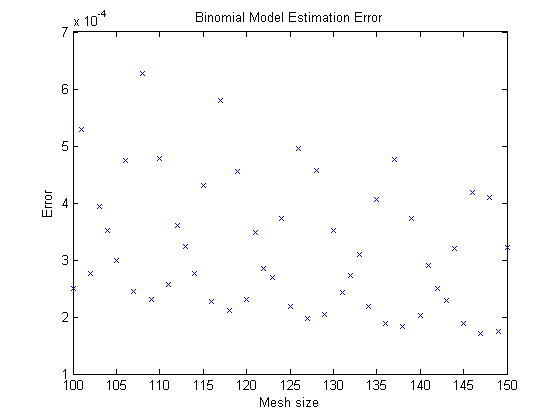
\includegraphics[width=0.5\textwidth]{fig01.png}
\caption{\label{fig:fig01}Plot of errors}
\end{figure}

\item Prices of the following European options:\\
Binary Cash-or-nothing Call: 0.012060\\
Binary Cash-or-nothing Put: 0.929704\\
Binary Asset-or-nothing Call: 0.133363\\
Binary Asset-or-nothing Put: 4.866637\\

\end{enumerate}

\pagebreak

\item Problem 8\\
\begin{enumerate}
\item It gives a symmetric recombining tree.\\

\item From $e^{r\dd t}=pu+(1-p)d$,
\[e^{-r\dd t}=\frac{1}{pu+(1-p)d}\]
From $e^{2r\dd t+\sigma^2\dd t}=pu^2+(1-p)d^2$,
\[e^{(r+\sigma^2)\dd t}=e^{-r\dd t}(pu^2+(1-p)d^2)=\frac{pu^2+(1-p)d^2}{pu+(1-p)d} \]
Given $ud=\gamma$, let $\beta=\frac{1}{2}\lb\gamma e^{-r\dd t}+e^{(r+\sigma^2)\dd t}\rb=\frac{1}{2}\lb\frac{ud}{pu+(1-p)d}+\frac{pu^2+(1-p)d^2}{pu+(1-p)d}\rb=\frac{1}{2}\lb\frac{pu^2+ud+(1-p)d^2}{pu+(1-p)d}\rb$
\begin{eqnarray*}
u-\beta&=&u-\frac{1}{2}\lb\frac{pu^2+ud+(1-p)d^2}{pu+(1-p)d}\rb\\
&=&\frac{2pu^2+2(1-p)ud-pu^2-ud-(1-p)d^2}{2(pu+(1-p)d)}\\
&=&\frac{pu^2+(1-2p)ud-(1-p)d^2}{2(pu+(1-p)d)}\\
&=&\sqrt{\frac{(pu^2+(1-2p)ud-(1-p)d^2)^2}{4(pu+(1-p)d)^2}}\\
&=&\sqrt{\frac{p^2u^4+(2p-4p^2)u^3d+(6p^2-6p+1)u^2d^2+(-4p^2+6p-2)ud^3+(1-p)^2d^4}{4(pu+(1-p)d)^2}}\\
&=&\sqrt{\frac{(pu^2+ud+(1-p)d^2)^2-4ud(pu+(1-p)d)^2}{4(pu+(1-p)d)^2}}\\
&=&\sqrt{\frac{(pu^2+ud+(1-p)d^2)^2}{4(pu+(1-p)d)^2}-ud}\\
&=&\sqrt{\beta^2-\gamma}
\end{eqnarray*}
Therefore, $u-\beta=\sqrt{\beta^2-\gamma}$, which gives $u=\beta+\sqrt{\beta^2-\gamma}$

\item Since $ud=\gamma$,\\
\begin{math}
S_0u^{\frac{M}{2}}d^{\frac{M}{2}}=K\\
(ud)^{\frac{M}{2}}=\frac{K}{S_0}\\
\gamma^{\frac{M}{2}}=\frac{K}{S_0}\\
\frac{M}{2}\ln\gamma=\ln\frac{K}{S_0}\\
\ln\gamma=\frac{2}{M}\ln\frac{K}{S_0}\\
\gamma=\exp\lb\frac{2}{M}\ln\frac{K}{S_0}\rb
\end{math}

\end{enumerate}
\end{enumerate}
\end{document}
